\begin{figure}[!htbp]
		\centering
		%\resizebox{\textwidth}{!}{%
			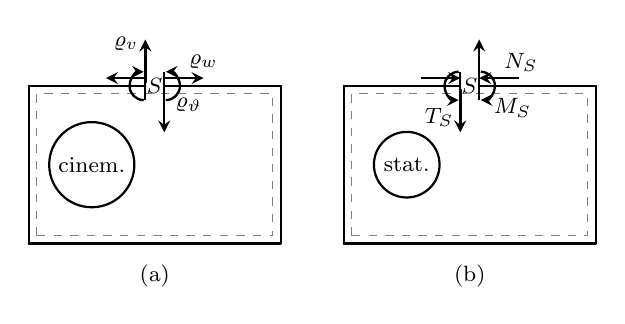
\begin{tikzpicture}[
				>=stealth, line width=0.8pt,
				trave/.style={line width=0.80pt, line cap=round, line join=round, black},
				taglio/.style={line width=0.8pt, black},    
				distor/.style={->, >=stealth, line width=0.9pt, black},
				sollec/.style={->, >=stealth, line width=0.9pt, black},
				etichetta/.style={circle, draw=black, inner sep=2.5pt,	line width=0.8pt, font=\footnotesize}]
				
				%% ===============================================================
				%% PANNELLO (a) — cinematico: tre distorsioni in S
				%% ===============================================================
				\begin{scope}[xshift=0cm, yshift=0cm]
					
					\def\W{3.2}
					\def\H{2.0}
					\def\dt{0.12}      %% mezza-larghezza dell'interruzione
					\def\el{0.18}      %% mezza-lunghezza del trattino trasversale
					
					\pgfmathsetmacro{\xS}{\W*0.5}      %% ascissa del taglio
					
					%% --- rettangolo con lato superiore interrotto in xS ---
					\draw[trave] (0,\H) -- ({\xS-\dt},\H);     %% lato sup. sinistro
					\draw[trave] ({\xS+\dt},\H) -- (\W,\H);    %% lato sup. destro
					\draw[trave] (0,0) -- (\W,0);              %% lato inferiore
					\draw[trave] (0,0) -- (0,\H);              %% lato sinistro
					\draw[trave] (\W,0) -- (\W,\H);            %% lato destro
					
					%% tratteggio della fibra inferiore: lato interno dell'anello
					\def\df{0.10}      %% distanza del tratteggio dal lato della trave
					\draw[dashed, thin, gray]
					({\df},{\df}) rectangle ({\W-\df},{\H-\df});
					
					%% --- trattini trasversali del taglio ---
					\draw[taglio] ({\xS-\dt},{\H-\el}) -- ({\xS-\dt},{\H+\el});
					\draw[taglio] ({\xS+\dt},{\H-\el}) -- ({\xS+\dt},{\H+\el});
					
					%% --- etichetta S in alto a destra del taglio ---
					\node[font=\footnotesize] at (\xS,\H) {$S$};
					
					%% --- varrho_w: due frecce orizzontali antagoniste SOPRA la trave ---
					%% (assiale: si avvicinano alle due facce dall'esterno)
					\pgfmathsetmacro{\yw}{\H+0.10}
					\def\dw{0.50}
					\draw[distor] (\xS-\dt,\yw) -- (\xS-\dw-\dt,\yw);
					\draw[distor] (\xS+\dt,\yw) -- (\xS+\dw+\dt,\yw);
					\node[font=\footnotesize, right=3pt] at (\xS+0.2,\yw+0.2)	{$\varrho_w$};
					
					%% --- varrho_v: due frecce verticali antagoniste,
					%%     attaccate agli estremi delle due facce ---
					%% (trasversale: una faccia scende, l'altra sale)
					\def\dv{0.55}
					\def\gv{0.04}      %% gap fra trattino-faccia e inizio freccia
					%% sulla faccia S^- (a sinistra del taglio): freccia verso l'alto
					\draw[distor] ({\xS-\dt},{\H+\gv}) -- ({\xS-\dt},{\H+\gv+\dv});
					%% sulla faccia S^+ (a destra del taglio): freccia verso il basso
					\draw[distor] ({\xS+\dt},{\H-\gv}) -- ({\xS+\dt},{\H-\gv-\dv});
					\node[font=\footnotesize, right=2pt] at ({\xS-\dt-0.6},{\H+\gv+\dv*0.9}) {$\varrho_v$};
					
					%% --- varrho_vartheta: due semiarchi antagonisti, sopra le facce ---
					\pgfmathsetmacro{\ya}{\H}      %% centro dei semiarchi
					\draw[->, >=stealth, line width=0.85pt]
					({\xS-0.14},{\ya-0.18}) arc (270:90:0.18);
					\draw[->, >=stealth, line width=0.85pt]	({\xS+0.14},{\ya-0.18}) arc (-90:90:0.18);
					\node[font=\footnotesize, right=1pt] at ({\xS+0.10},\ya-0.24) {$\varrho_\vartheta$};
					
					%% --- etichetta diagramma (in angolo interno dell'anello) ---
					\node[etichetta] at (\W*0.25,\H*0.5) {cinem.};
					
					%% --- etichetta pannello ---
					\node[below=4pt, font=\footnotesize] at (\W/2,0) {(a)};
				\end{scope}
				
				%% ===============================================================
				%% PANNELLO (b) — statico: tre caratteristiche in S come coppie
				%%                autoequilibrate, parametricamente libere
				%% ===============================================================
				\begin{scope}[xshift=4cm, yshift=0cm]
					
					\def\W{3.2}
					\def\H{2.0}
					\def\dt{0.12}      %% mezza-larghezza dell'interruzione
					\def\el{0.18}      %% mezza-lunghezza del trattino trasversale
					
					\pgfmathsetmacro{\xS}{\W*0.5}      %% ascissa del taglio
					
					%% --- rettangolo con lato superiore interrotto in xS ---
					\draw[trave] (0,\H) -- ({\xS-\dt},\H);     %% lato sup. sinistro
					\draw[trave] ({\xS+\dt},\H) -- (\W,\H);    %% lato sup. destro
					\draw[trave] (0,0) -- (\W,0);              %% lato inferiore
					\draw[trave] (0,0) -- (0,\H);              %% lato sinistro
					\draw[trave] (\W,0) -- (\W,\H);            %% lato destro
					
					%% tratteggio della fibra inferiore: lato interno dell'anello
					\def\df{0.10}      %% distanza del tratteggio dal lato della trave
					\draw[dashed, thin, gray]
					({\df},{\df}) rectangle ({\W-\df},{\H-\df});
					
					
					%% --- trattini trasversali del taglio ---
					\draw[taglio] ({\xS-\dt},{\H-\el}) -- ({\xS-\dt},{\H+\el});
					\draw[taglio] ({\xS+\dt},{\H-\el}) -- ({\xS+\dt},{\H+\el});
					
					%% --- etichetta S in alto a destra del taglio ---
					\node[font=\footnotesize] at (\xS,\H) {$S$};
					
					%% --- varrho_w: due frecce orizzontali antagoniste SOPRA la trave ---
					%% (assiale: si avvicinano alle due facce dall'esterno)
					\pgfmathsetmacro{\yw}{\H+0.10}
					\def\dw{0.50}
					\draw[distor] (\xS-\dw-\dt,\yw) -- (\xS-\dt,\yw);
					\draw[distor] (\xS+\dw+\dt,\yw) -- (\xS+\dt,\yw);
					\node[font=\footnotesize, right=3pt] at (\xS+0.2,\yw+0.2)	{$N_S$};
					
					%% --- T_S due frecce verticali antagoniste,
					%%     attaccate agli estremi delle due facce ---
					%% (trasversale: una faccia scende, l'altra sale)
					\def\dv{0.55}
					\def\gv{0.04}      %% gap fra trattino-faccia e inizio freccia
					\draw[distor] ({\xS-\dt},{\H-\gv}) -- ({\xS-\dt},{\H-\gv-\dv});
					\draw[distor] ({\xS+\dt},{\H+\gv}) -- ({\xS+\dt},{\H+\gv+\dv});
					%\draw[distor] ({\xS+\dt},{\H-\gv}) -- ({\xS+\dt},{\H-\gv-\dv});
					\node[font=\footnotesize, right=2pt] at ({\xS-\dt-0.65},{\H+\gv-\dv*0.8}) {$T_S$};
					
					%% --- M_S: due semiarchi antagonisti, ---
					\pgfmathsetmacro{\ya}{\H}      %% centro dei semiarchi
					\draw[<-, >=stealth, line width=0.85pt]	({\xS-0.14},{\ya-0.18}) arc (270:90:0.18);
					\draw[<-, >=stealth, line width=0.85pt]	({\xS+0.14},{\ya-0.18}) arc (-90:90:0.18);
					\node[font=\footnotesize, right=1pt] at ({\xS+0.14},\ya-0.28) {$M_S$};
					
					%% --- etichetta diagramma (in angolo interno dell'anello) ---
					\node[etichetta] at (\W*0.25,\H*0.5) {stat.};
					
					%% --- etichetta pannello ---
					\node[below=4pt, font=\footnotesize] at (\W/2,0) {(b)};
				\end{scope}
				
			\end{tikzpicture}%
			%}%
		\caption{Trave biconnessa con taglio ideale in $S$:
			rappresentazione duale delle tre grandezze cinematiche
			e statiche associate al vincolo di rigidità.
			(a)~Le tre distorsioni $\varrho_w$, $\varrho_v$,
			$\varrho_\vartheta$ come scarti cinematici fra le
			due facce $S^-$ ed $S^+$.
			(b)~Le tre caratteristiche della sollecitazione
			$N(S)$, $T(S)$, $M(S)$ come azioni interne agenti
			sulle stesse facce. Le grandezze sono disegnate nel
			verso positivo secondo le convenzioni di segno}
		\label{fig:biconnessa_dualita}
	\end{figure}
